\chapter{Design}
\label{sec:design}

% Ist das zentrale Kapitel der Arbeit. Hier werden das Ziel sowie die
% eigenen Ideen, Wertungen, Entwurfsentscheidungen vorgebracht. Es kann
% sich lohnen, verschiedene Möglichkeiten durchzuspielen und dann
% explizit zu begründen, warum man sich für eine bestimmte entschieden
% hat. Dieses Kapitel sollte - zumindest in Stichworten - schon bei den
% ersten Festlegungen eines Entwurfs skizziert werden.
% Es wird sich aber in einer normal verlaufenden
% Arbeit dauernd etwas daran ändern. Das Kapitel darf nicht zu
% detailliert werden, sonst langweilt sich der Leser. Es ist sehr
% wichtig, das richtige Abstraktionsniveau zu finden. Beim Verfassen
% sollte man auf die Wiederverwendbarkeit des Textes achten.

% Plant man eine Veröffentlichung aus der Arbeit zu machen, können von
% diesem Kapitel Teile genommen werden. Das Kapitel wird in der Regel
% wohl mindestens 8 Seiten haben, mehr als 20 können ein Hinweis darauf
% sein, daß das Abstraktionsniveau verfehlt wurde.

%%%%%%%%%%%%%%%%%%%%%%%%%%%%%%%%%%%%%%%%%%%%%%%%%%%%%%%%%%%%%%%%%%%%%%%%%%%%%%%%
%                                                                              %
% MOTIVATION AND REQUIREMENTS                                                  %
%                                                                              %
%%%%%%%%%%%%%%%%%%%%%%%%%%%%%%%%%%%%%%%%%%%%%%%%%%%%%%%%%%%%%%%%%%%%%%%%%%%%%%%%
\section{Motivation}
\begin{itemize}
% Overall motivation of a communication layer
\item Parallel computers are stricly necessary in scientific community
\item Parallel computers are compute clusters
  \ref{sec:cluster} with a very homogeneous layout, in which the nodes
  are connected by a abitrary network.  Usually application domain is
  decomposed \ref{sec:domain_decomposition} in smaller chunks
  of work and then distributed onto the homogenous network of nodes on
  the cluster.  So to speak a very heterogeneous phyisical simulation
  is mapped onto a homogeneous compute architecture.

  This is fine as long the simulation is not changing to much during
  runtime. Thus every node stays utilized. But instead real world
  simulations are changing over time. The workload could increase
  globally or only locally on some subdomains of the simulation
  volume.

  This leads to an unbalanced load during the simulation and therefore
  to unutilized ressource of the compute cluster. In this cases it
  could make sense to start some new domain decomposition or it could
  also make sense to move whole subdomains from one node to another.

  This all needs a powerful communication layer which is flexibel
  enough to support such rebalancing of workload. Common cluster
  communication frameworks are not able to fullfill these
  requirements. They are usually static in their distribution and do
  not satisfy our needs.

  \todo{State out that communication layer should be exchangeable}

\item PIConGPU \ref{sec:picongpu} is even harder because of an
  hierarchicle memory architecture.
\item NUMA architecture will crow even harder
\end{itemize}

Fact is, that the communication hardware layout is fixed. The access
to the hardware is represented by CALs (See \ref{sec:cal}) and these
are connected in the simplest case by an fully connected network, thus
every peer can send messages to every other peer. Therefore a network
on top of the CALs has to be established.

It is a very important property to be able to explicitly map the
communication topologie of the application onto the communication
hardware.

In the first place it should gives the application the possibility to
be optimized on special charakteristics of the compute cluster. For
example could vertices that need to communicate very intensively with
each other can be mapped on neighboring nodes or even onto the same
node. Which makes communication more efficient.

Besides it should be possible to change the mapping of the
communication topologie onto the communication hardware in
runtime. This is important when thinking of occuring unbalanced load
during the run of the application.

The communication is abstracted from the actual communication layer by
the CAL and the communicaiton topologie is modeled with a graph and
then maped onto the CAL.

% Requirements
\subsection{Requirements}
To be able to model such complex and heterogeneous topologies the
following components are required:

\begin{itemize}
\item Communication abstraction layer, which introduce an abstraction
  from existig communication layers.
\item Description of the communication topology
\item Possibility to communicate inside the physical domain
\item Mapping of communiation topology onto the hardware topology
\end{itemize}

%%%%%%%%%%%%%%%%%%%%%%%%%%%%%%%%%%%%%%%%%%%%%%%%%%%%%%%%%%%%%%%%%%%%%%%%%%%%%%%%
%                                                                              %
% ANALYSIS OF PIConGPU CODE                                                    %
%                                                                              %
%%%%%%%%%%%%%%%%%%%%%%%%%%%%%%%%%%%%%%%%%%%%%%%%%%%%%%%%%%%%%%%%%%%%%%%%%%%%%%%%
\section{Analysis of PIConGPU-Code}
\begin{itemize}
  \item How does the communication topologie looks like ?
  \item What are the different levels of communication ?
  \item What kind of communcation layer is used ?
  \item How is Communication implemented in PIConGPU ?
\end{itemize}

%%%%%%%%%%%%%%%%%%%%%%%%%%%%%%%%%%%%%%%%%%%%%%%%%%%%%%%%%%%%%%%%%%%%%%%%%%%%%%%%
%                                                                              %
% COMMUNICATION ABSTRACTION LAYER                                              %
%                                                                              %
%%%%%%%%%%%%%%%%%%%%%%%%%%%%%%%%%%%%%%%%%%%%%%%%%%%%%%%%%%%%%%%%%%%%%%%%%%%%%%%%
\section{Abstraction from Existing Communication Layers}
\todo{Wie trägt komponente bei motivation zu erfüllen}

% Motivation for communication abstraction
Applications can be interconnected by vast variety of communication
libraries. But it can not be assumed that every cluster system
supports every communication library on the market.  Thus, the
abstraction from existing communication libraries is a fundamental
property for a flexibel and portable application.

Even though, that there are existing standards for communication in
cluster systems, the world of computer science is subject to constant
change. Thus the possibility to exchange the used communication layer
without changing the interface to this layer, is a precondition for
future applications in distributed computing.

The challange is to provide a very general interface, that is able to
map varying communication libraries onto it. This interface should not
be modeled from the scratch, instead it should remind the interface
user on known communication methods. It should be deployable into existing
applications by replacing the actual communication library without
changing the understanding of the fundamental way to communicate in
this application.

This section presents the design of a generic communication layer
which fulfils the before discussed requirements.

% Brief CAL description
\subsection{Communication Abstraction Layer (CAL)}
\label{sec:cal}
The \textit{Communication Abstraction Layer}, shortly \textit{CAL}, is
a generic interface that provides access to a varity of communication
libraries. The libraries are available as adapters, which can be
configured at compile time (Figure \ref{fig:cal}).

\begin{figure}[H]
  \centering 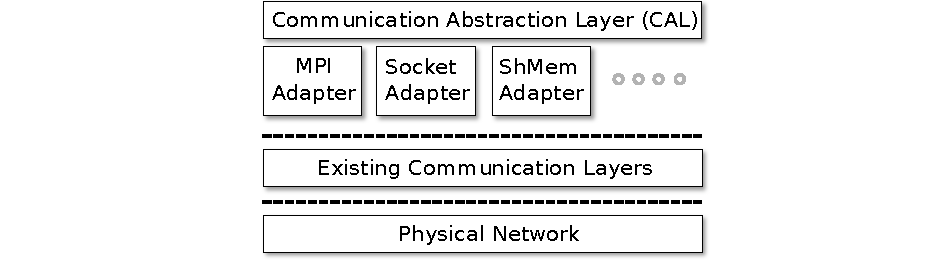
\includegraphics[width=\textwidth]{graphics/30_cal}
  \caption{Communication Abstraction Layer (CAL)}
  \label{fig:cal}
\end{figure}

Using the CAL instead of a concrete communication library has the
advantage that in the case of a changing communication environment
(e.g migrating to another cluster) only the adapter has to be
exchanged and the application has to be recompiled, but the CAL does
not change.

\subsection{Addressing of Peers}
% CAL virtual addressing
Communication libraries come with their own address schema, which can
be quiete different. Socket based systems address their peers by ip
addresses, where MPI based systems address their processes by ranks.
These diverse ways to address peers in a network need to be translated
to an unified address space. Each CAL provides a virtual address
which is an unique identifier for its peer in the adapters network.

The address space of the virtual address are natural numbers in 
the range from 0 to the number of peers minus one. This addressing
schema is the simplest way and satifies the needs of the actual design.

% CAL interface
\subsection{Communication Interface}
\label{sec:cal_comm}
% Peer2Peer Operations
\subsubsection{Peer to Peer Operations}

In the first place the CAL provides peer-to-peer communication. That
are basic communication operations to send and receive abitrary data
between two peers. These operations are available both blocking and
non-blocking. Non-blocking operations return an event, that can be
queried whether it has finished or it can be waited until it has
finished. The interface is influenced by existing communication
libraries that all share a common interface ( e.g.boost::mpi,
boost::asio, ZMQ). The core interface for sending and receiving data:

\begin{itemize}
  \item send(destination, tag, data)
  \item recv(source, tag, data)
\end{itemize}

\begin{description}
\item[Data] \hfill \\
  The data that should be transmitted to
  another peer or that should be received from another peer.  The data
  object should provide a function data() that returns the pointer to a
  contigiuous memory area and a function size() that returns the size
  of the object. The STL sequence containers std::vector and
  std::array allready support these functions at least since C++ version
  C++11.
\item[Destination / Source] \hfill \\
  This is the virtual address of the sending or receiving peer.
\item[Message Tag] \hfill \\
  The message tag is an unsigned interger that gives
  a message a meaning similar to headers of communication
  protocols. Thus, it helps a peer to distinguish between messages of
  the same sending peer.
\end{description}

It is not planed in the actual design that the CAL provides routing
abilities. Peers have to be connected directly by the network of the
adapter. No routing makes it also impossible to forward data between
different adapters of the CAL. Thus a specific CAL only provides a
single adapter. But several CALs can be used with different adapters
to communcate on several networks. In such a scenario the routing can
be implemented on top of the CAL by the library user.future work could
also implement an routing underneath the CAL to reach also not
directly connected peers automatically. This kind of routing
could also connect two different adatpers with each other.

% Context
\subsubsection{Grouping of peers}
\label{sec:cal_context}
The CAL also supports a grouping of peers of the same adapter. Such a
group of peers will be called context. A context is the base for
algorithms with more than 2 participating peers. These operations
where introduced as collective operations (Section \ref{sec:collectives}). 
\todo{create context + get global context + context interface}

% Collectives Operations
\subsubsection{Collective Operations}
\label{sec:cal_collective}
There is a large number of collective operations known to the
parallel computation commmunity. The CAL only provides the most
important ones with respect to its objective platform PIConGPU \ref{sec:picongpu}:

\begin{itemize}
\item gather(root, context, send, recv)\\
  This operation collects data of the same size from
  every peer in the context. The collected data will be
  received from the root peer.
  %\item gatherUnequal(root, context, send, recv, recvCount)
\item allGather(context, send, recv)
  %\item allGatherUnequal(context, send, recv, recvCount)
\item scatter(root, context, send, recv)
  This operation distributes varying data of the same size from the root peer to
  all other peers of the context.
\item allScatter(context, send, recv)

\item reduce(root, context, operation, send, recv)
  \todo{more about reduce}
  This operation reduces the data from every peer of a context by
  a binary function.

\begin{itemize}
  \item Binary Function
    A binary function in general, takes two arguments of abitrary type and
    returns a value of abitrary type. Usually bost input arguments and
    return value have the same type. The C++ STL allready provides
    a handfull of binary functions in the functional header. Not provides
    functions can be easily created (See \ref{list:binary_functions}
    as example).

    \begin{lstlisting}[language=C++, breaklines=false]
      \label{list:binary_function}
      template<typename T>
      struct add : public std::binary_function<T, T, T>
      {
        const T& operator()(const T& x, const T& y) const
        {
          return x + y;
    \end{lstlisting}
  \end{itemize}

\item allReduce(context, operation, send, recv)

\item broadcast(root, context, data)
  This operation distributes data from the root peer to
  all other peers of the context.
\item syncronize(context)
  This operation synchronizes the control flow of all peers of the context.
\item createContext(peers, context)
  This operation creates a new context from the context. Such a smaller
  group of peers can be created.
\end{itemize}

\todo{future work}
Future work will be the support of collective operations over the borders
of different adapters in the case that the CAL supports more than one adapter
being instanciated.


%%%%%%%%%%%%%%%%%%%%%%%%%%%%%%%%%%%%%%%%%%%%%%%%%%%%%%%%%%%%%%%%%%%%%%%%%%%%%%%%
%                                                                              %
% GRAPH                                                                        %
%                                                                              %
%%%%%%%%%%%%%%%%%%%%%%%%%%%%%%%%%%%%%%%%%%%%%%%%%%%%%%%%%%%%%%%%%%%%%%%%%%%%%%%%
\section{Modeling of the Application Domain}
\label{sec:graph}
Domain decomposed applications are seperated into a set of
subdomains. The decomposition method also defines the relationship
between subdomains. Often this relationship is hardcoded into the
applications source code. A Change of the decomposition method or the
applications domain therefore also implies a change in the
applications algorithm. This reduces the flexibilty of application.

A more elegant way is to explicitly model the relationships between
the subdomains. The most general method to model such correlations is
a graph \cite{ref:graph}. It has the advantage that a algorithm can be
implemented on top of the graph domain description. Thus a change in
the application domain only implies a different graph, but not
necessarily an adapted algorithm.

From the mathematical background, a graph is a pair of vertices and
edges. Edges are pairs of vertices. So to speak, a graph represents a
set of objects, where some of these objects are connected by links.

% directed cycle multi graph
Keeping in mind that a wide range of application should be possible to
model, the graph is not very restricted. Vertices are connected by
directed edges. Loops and multiple edges between two vertices are
allowed (Figure \ref{fig:graph}). The mathematical expression for this
kind of graph is quiver \cite{ref:quiver}

\begin{figure}[H]
  \centering 
\includegraphics[width=\textwidth]{graphics/30_graph}
  \caption{ A directed cycle multi graph with vertices A, B and edges
    1, 2, 3.  }
  \label{fig:graph}
\end{figure}

\todo{Is an interface to the graph needed here?}

\subsection{Graph Properties}
A graph alone is just the representation of the connected vertices,
but has no connection to the application domain. The connection
usually only exists in the head of the programmer.

For this purpose the concept of graph properties is introduced. A
property provides abitrary subdomain information and can be bound to
vertices and edges (Figure \ref{fig:property}). Vertices and Edges of
the same graph share respecively the same type of property. A graph
annoted with properties is significantly more meaningful and thus
helps to keep the connection of the application domain and the graph.

\begin{figure}[H]
  \centering 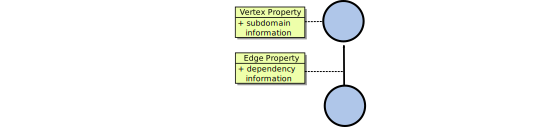
\includegraphics[width=\textwidth]{graphics/30_property}
  \caption{A graph with both vertex and edge properties. The vertex
    property primarily describe a subdomain. the edge property
    describe the relationship between subdomains.}
  \label{fig:property}
\end{figure}

A Property can also be used to create a connection between a pair of
graphs. Thus a modeling of hiararchical domains is also possible.  A
later example will make use of this hierarchical modelation (Section
\ref{sec:gol}).


\subsection{Modeling Game of Life as a graph}
\label{sec:gol}
To give an example figure \ref{fig:gol} models the Game of Life (GoL)
\cite{ref:gol} world by a graph. GoL simulates the evolution of a set
of cells for unlimited timesteps. A cell has a status which is either
alive or not alive and the status of the next evolution step is
calculated by rules including the status information of the
neighboring cells.GoL was modeled straight forward.  Every cell of the
GoL world is represented by a vertex and neighboring cells are
connected by an edge. Each vertex has the property cell which only
contains the status of the cell.

\begin{figure}[H]
  \centering 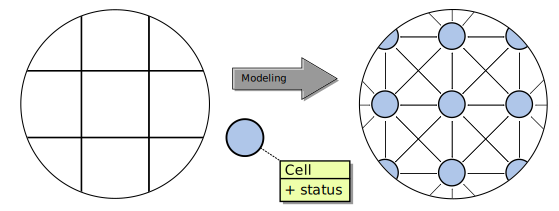
\includegraphics[width=\textwidth]{graphics/30_gol}
  \caption{Cut-out of a Game of Life world (on the left) was modeled
    as a graph (on the right). Each Vertex is described by the vertex
    property cell, containing the status information of the cell.}
  \label{fig:gol}
\end{figure}

% Partitioned graph
The graph in figure \ref{fig:gol} models the relationship of the
smallest entities of GoL, the cells itself. It is a unification of the
data representation of the cells and the communication dependencies
between the cells. This might be not very efficient when this graph is
the foundation for a distributed computing application. To take it to
extremes, a single cell could be calculated by its own process and the
cell status could be exchanged by inter-process communication
. This might not be the most efficient implementation of GoL,
because a single process can compute considerably more cells.

Figure \ref{fig:gol_bundle} partitions the GoL graph by bundling
multiple vertices together and models a partioned graph. These Bundles are
connected by edges when the cells inside the bundles where connected
before. While the GoL graph represents the GoL cells in detail, the
partitioned graph represents dependencies of bundled cells. Thus
the properties of the partioned graph changed such that bundles
have store the cells they bundle and edges refer to neighboring
cells.

\begin{figure}[H]
  \centering 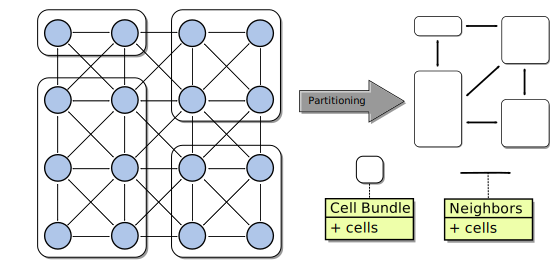
\includegraphics[width=\textwidth]{graphics/30_gol_bundle}
  \caption{The GoL graph is partitioned by bundling multiple
    cells. The properties of the partioned graph have changed, such
    that the vertex property contains the cells of a bundle, while the
    edge property contains information about neighboring cells.}
  \label{fig:gol_bundle}
\end{figure}

The partitioned graph could be used as foundation to distribute GoL to
multiple devices on a cluster. Each bundle could be computed by an own
device. 

% Graph partitioning optimitsation
The creation of bundles that are optimized to a minimum of connections
and a maximum of ressource utilization is the topic graph partitioning
algorithms. But the modeling of optimal partitioned graphs is not part
of this work.

\todo{subgraphs!}

%%%%%%%%%%%%%%%%%%%%%%%%%%%%%%%%%%%%%%%%%%%%%%%%%%%%%%%%%%%%%%%%%%%%%%%%%%%%%%%%
%                                                                              %
% GRAPH-BASED VIRTUAL OVERLAY NETWORK                                          %
%                                                                              %
%%%%%%%%%%%%%%%%%%%%%%%%%%%%%%%%%%%%%%%%%%%%%%%%%%%%%%%%%%%%%%%%%%%%%%%%%%%%%%%%
\section{Graph-Based Virtual Overlay Network (GVON)}
%% Requirements
The objective is to establish a communication layer within the
applications domain. Such that communication between subdomains of the
application can be represented. Therefore, this section introduces a
graph-based virtual overlay network (GVON), that is based on the graphs and the
CAL introduced in the previous sections \ref{sec:graph} and
\ref{sec:cal}). 

The graph does only provide domain specific information.  It can be
used as a blueprint for the virtual network topologie.  Thus
communication operations are provided by the CAL and the virtual
network is described by a graph (Figure \ref{fig:gvon})

\begin{figure}[H]
  \centering 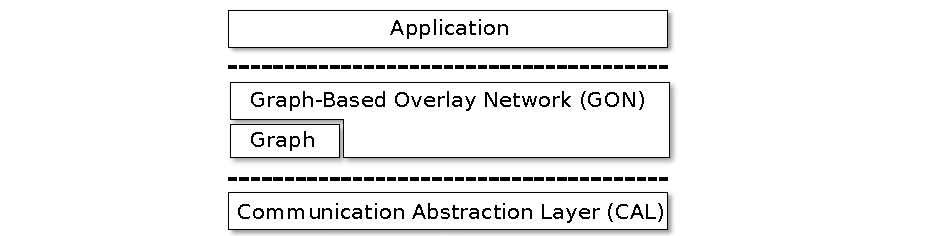
\includegraphics[width=\textwidth]{graphics/30_gon}
  \caption{The Graph-based virtual overlay network provides communication
    functionality based on the CAL}
  \label{fig:gvon}
\end{figure}

It is important that all peers that want to take part on the
communication of the GVON need to know the same graph. In order to
ensure that, the graph can be constructed in parallel by all peers,
loaded from the same file of a distributed file system or could even
be delivered by a master peer.

%% Process of announce
\subsection{Mapping of the GVON onto the CAL}
\label{sec:mapping}
The connection between the CAL and a graph is maintained through a
mapping of vertices to peers (vertex map). In the context of an
overlay network, a vertex is interpreted as a virtual peer of the GVON,
edges between adjacent vertices indicate that the virtual peers are
able to communicate with each other. The mapping of vertices to peers
is a joint process of all peers that want to take part at the
communication based on a specific graph.

The first phase is the distribution of the vertices of the graph to
the peers (Figure \ref{fig:gon_mapping}). This has the meaning that a
peer is responsible for the communication of these vertices. The peer
will be called host of the its hosted vertices. A peer is responsible
either for zero, one or more vertices, so to speak it is also possible
that one peer hosts all vertices and communicates finally always with
itself.

\begin{figure}[H]
  \centering 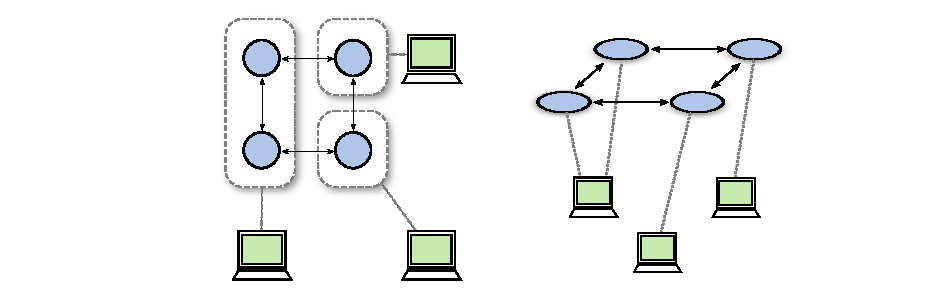
\includegraphics[width=\textwidth]{graphics/30_gon_mapping}
  \caption{All vertices of a graph are distributed onto 3 peers. The vertices
  are not distributed evenly, thus one peer is host for 2 vertices.}
  \label{fig:gon_mapping}
\end{figure}

There are a varity of methods to distribute the vertices of a graph to
the peers of a network. It could be done totally randomized, round
robin or even dictated by some master peer. The distribution behavior
is defined be the user of the library and might be object for further
optimization.

In the next phase the peers announce their hosted vertices to all
other peers. This means that every peer receives from every other peer
a list of its hosted vertices. This mapping acts as a kind of a
nameservice. It can be queried for the hosting peer of a
vertex. Furthermore the GVON maps the announced graph to a context
\ref{sec:cal_context} containing all peers attended to the
announcement process (graph map). Communication can now be established
on basis of this mappings.

% Communication
\subsection{Communication within the GVON}
The application has the view, that it really is exchaning messages
between the vertices of the graph and the GVON is taking care, that
the messages are reaching the correct vertex host. Thus this is
finally the level of abstraction that the application interacts with.

The GVON provides similar functionality like the introduced operations
in the CAL. Thus both peer to peer and collective operations are
provided.

% GVON P2P
A peer to peer operations within the GVON involves exchanging data
between adjacent vertices over a specific edge of a specific graph.
Thus the function interface looks like the following.

\begin{itemize}
  \item send(graph, destination vertex, edge, data)
  \item recv(graph, source vertex, edge, data)
\end{itemize}

The GVON has the task to resolv both the context of a graph and the
host of the source or the destination vertex. This information are
quieried from the vertex and graph map. When this information is
resolved the programm flow is handed over to the CAL, that trasmits or
receives data.

% GVON collectives
Operations between all vertices of a graph can be performed as
collective operations \ref{sec:collectives}. A host needs to
perform the collective operation for all its hosted vertices,
otherwise it blocks the execution of the operation. Yet again
the result of the collective is reveived by some root vertex
or by all vertices of the graph.

The collective operation is first executed locally for all hosted
vertices of each peer. Then it is further handled by the CAL and
transmitted to the receiver(s). Figure \ref{fig:gon_collective} shows
a gather operation on the same graph and mapping of figure
\ref{fig:gon_mapping}. For each vertex of the graph a gather operation
is executed.

\begin{figure}[H]
  \centering 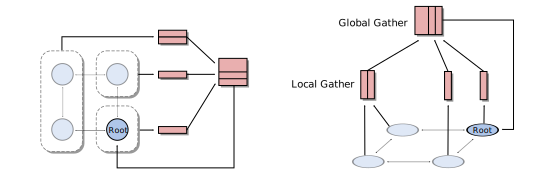
\includegraphics[width=\textwidth]{graphics/30_gon_collective}
  \caption{Gather operation of the GVON. Data is first locally for
    each peer and then globally collected. Finally the collected data
    is transmitted to the root vertex.}
  \label{fig:gon_collective}
\end{figure}

Further collective operations provided by the GVON are the 
following :

\begin{itemize}
\item Gather - Vertices on the same host collect data local first and
  then use the collective gather provided by the communicator
\item Reduce - Vertices on the same host reduce data local first and
  then use reduce provided by the communicator.
\item Synchronize - This is a barrier function which lets the host
  wait for all others host that are contributing to a special graph.
\end{itemize}

%% Remapping of vertices
\subsection{Reannounce Vertices}
The communication hardware and communication topolgie is now
seperated, therefor it is possible to change the mapping from
vertices to peers at runtime. That can be necessary when load of an
application is getting inbalanced during runtime.

Like in section \ref{sec:mapping}, it is again necessary to perform two steps for the remapping;
distributing and announncing. Thus vertices are distributed by some
rule and then announced. Depending on the application, also 
vertex data has to be transfered to hosts with new vertices.

The remapping can be done both local and global. For local remapping
only peers that host a vertex that is connected to a remapped vertex
are involved. A global remapping is very similar to an inital mapping
and involves all peers (or even more).

\todo{remapping figure}


%%%%%%%%%%%%%%%%%%%%%%%%%%%%%%%%%%%%%%%%%%%%%%%%%%%%%%%%%%%%%%%%%%%%%%%%%%%%%%%%
%                                                                              %
% ETC                                                                          %
%                                                                              %
%%%%%%%%%%%%%%%%%%%%%%%%%%%%%%%%%%%%%%%%%%%%%%%%%%%%%%%%%%%%%%%%%%%%%%%%%%%%%%%%

\subsection{Requirements for the upcoming generation of super computers}
\begin{itemize}
\item Run picongpu on xeon phi in native mode
\item Exchangeable communication layer to be portable / ready for the
  upcoming generation of acceleration devices
\end{itemize}


The during this thesis developed communication layer was leaded by the
needs of PIConGPU as an example application for high performance
computing on cluster systems.

The implementation of PIConGPU has some lack of abstraction for their
communication. Because there is no abstraction layer which hides the
MPI communication calls, which makes it impossible to exchange it.

Also the communication topology of the simulations is not be modeled
satisfying. Neighboring subdomains are directly addressed by their
ranks, thus changing the communication topology also leads to a lot of
changes in the algorithm.



\cleardoublepage

%%% Local Variables:
%%% TeX-master: "diplom"
%%% End:
